% \documentclass[letterpaper,12pt,oneside, draft]{book}
\documentclass[letterpaper,12pt,oneside]{book}
%%
%%  Gabarit de mémoire de maîtrise ou thèse de doctorat.
%%  Template for dissertations and theses @ Polytechnique Montreal.

%%  Normalement, il n'est pas nécessaire de modifier ce document
%%  sauf pour établir le langage (français ou anglais) et pour changer les noms des
%%  fichiers à inclure.
%%  Usually, this document needs to be modified only to set up the language (French or English)
%%  and to change the names of the files to include.
%%
%%  Version: 2018-07-31
%%
%%  Accepte les caractères accentués dans le document (UTF-8).

\makeatletter
\def\bstctlcite{\@ifnextchar[{\@bstctlcite}{\@bstctlcite[@auxout]}}
\def\@bstctlcite[#1]#2{\@bsphack
 \@for\@citeb:=#2\do{%
   \edef\@citeb{\expandafter\@firstofone\@citeb}%
   \if@filesw\immediate\write\csname #1\endcsname{\string\citation{\@citeb}}\fi}%
 \@esphack}
\makeatother

% CETTE COMMANDE ÉTABLIT LE LANGAGE DE LA THÈSE : ÉCRIRE french POUR UNE THÈSE EN FRANÇAIS
% THE NEXT COMMAND DETERMINES THE LANGUAGE OF THE THESIS: WRITE english FOR A THESIS IN ENGLISH
\newcommand\Langue{english}

% This command defines the school used, either centrale or poly
\newcommand\School{centrale}

\usepackage{ifthen}
\usepackage[utf8]{inputenc}
%%
%% Support pour l'anglais et le français (français par défaut).
%\usepackage[cyr]{aeguill}
\usepackage{lmodern}      % Police de caractères plus complète et généralement indistinguable visuellement de la police standard de LaTeX (Computer Modern).
\usepackage[T1]{fontenc}  % Bon encodage des caractères pour qu'Acrobat Reader reconnaisse les accents et les ligatures telles que ffi.

% le langage par défaut est le dernier de la liste, c'est-à-dire français
\ifthenelse{\equal{\Langue}{english}}{
	\usepackage[french,english]{babel}
}{
	\usepackage[english,french]{babel}
}

%%
%% Charge le module d'affichage graphique.
\usepackage{graphicx}
% \usepackage{epstopdf}  % Permet d'utiliser des .eps avec pdfLaTeX.
%%
%% Recherche des images dans les répertoires.
\graphicspath{{images/}}
\DeclareGraphicsExtensions{.pdf,.jpeg,.png}

%%
%% Un float peut apparaître seulement après sa définition, jamais avant.
\usepackage{flafter,placeins}
%%
%% Utilisation de natbib pour les citations et la bibliographie.
%\usepackage{natbib}
%%
%% Autres packages.
\usepackage[hyphens,spaces,obeyspaces]{url}
\usepackage{amsmath,color,soulutf8,longtable,colortbl,setspace,xspace,pdflscape,cite,amssymb}
%%
%% Support des acronymes.
\usepackage[nolist]{acronym}

\onehalfspacing                % Interligne 1.5.
%%
%% Définition d'un style de page avec seulement le numéro de page à
%% droite. On s'assure aussi que le style de page par défaut soit
%% d'afficher le numéro de page en haut à droite.
\usepackage{fancyhdr}
\fancypagestyle{pagenumber}{\fancyhf{}\fancyhead[R]{\thepage}}
\renewcommand\headrulewidth{0pt}
\makeatletter
\let\ps@plain=\ps@pagenumber
\makeatother
%%
%% Module qui permet la création des bookmarks dans un fichier PDF.
\usepackage{hyperref}
\usepackage{caption}  % Hyperlink on figure and not its title.
\usepackage{float}

\usepackage{amsthm}
\addto\captionsfrench{\renewcommand\proofname{Proof}}

\RequirePackage[chapter]{algorithm}
\usepackage{algpseudocode}

%% TIKZ

\usepackage{pgf,tikz,pgfplots,tikzit}
\pgfplotsset{compat=newest}
\usepackage{mathrsfs}
\usetikzlibrary{arrows}
\usetikzlibrary[patterns]

\makeatletter
\providecommand*{\toclevel@compteur}{0}
\makeatother

\usepackage{multirow}

\newcommand{\mathbbm}[1]{\text{\usefont{U}{bbm}{m}{n}#1}}

\usepackage[capitalize,nameinlink]{cleveref}[0.21]

%%
%% Définitions spécifiques au format de rédaction de Poly.
%% Here we define the Poly formatting.
\RequirePackage[\Langue]{MemoireThese}
%%
%% Définitions spécifiques à l'étudiant.
%% -----------------------------------
%% ---> À MODIFIER PAR L'ETUDIANT / TO BE MODIFIED BY THE STUDENT <---
%% -----------------------------------
%%
%% Commandes qui affichent le titre du document, le nom de l'auteur, etc.
\newcommand\monTitre{My fancy thesis title}
\newcommand\monTitreFR{Mon titre de thèse}
\newcommand\monPrenom{Mathieu}
\newcommand\monNom{Besançon}
\newcommand\monDepartement{Mathématiques et Génie Industriel}  % Department
\newcommand\maDiscipline{Mathématiques de l'Ingénieur} % The title of the degree
\newcommand\monDiplome{D}        % (M)aîtrise ou (D)octorat / (M)aster or Ph(D)
\newcommand\anneeDepot{2020}    % Year
\newcommand\moisDepot{Décembre}       % Month
\newcommand\monSexe{M}           % "M" ou "F" = Gender
\newcommand\PageGarde{O}         % "O" ou "N" = Yes or No
\newcommand\AnnexesPresentes{O}  % "O" ou "N". Indique si le document comprend des annexes. / If the thesis includes appendices = O Yes or N = No.
\newcommand\mesMotsClef{demand response, pricing, bilevel optimization, robust optimization}
\newcommand\mesMotsClefFR{réponse de la demande, tarification, optimisation biniveau, optimisation robuste}
%%
%%  DEFINITION DU / OF JURY
%%
%%  Pour la définition du jury, les macros suivantes sont definies:
%%  \PresidentJury, \DirecteurRecherche, \CoDirecteurRecherche, \MembreJury, \MembreExterneJury
%%
%%  Toutes les macros prennent 3 paramètres: Sexe (M/F), Nom, Prénom
%%  All the macros have 3 parameters: Sex (M/F), Last name, First name
\newcommand\monJury{
\PresidentJury{M}{}{}\\
\DirecteurRecherche{M}{}{}\\
\CoDirecteurRecherche{M}{}{}\\
\MembreJury{M}{}{}\\
\MembreExterneJury{F}{}{}
}

\newcommand\monJuryCentrale{
\begin{tabular}{lll}
	\textbf{Président} & Gilles Savard & Professeur, Polytechnique Montréal \\
	\textbf{Rapporteure} & Ivana Ljubic & Professeure, ESSEC \\
	\textbf{Rapporteur} & Martin Schmidt & Professeur, Universität Trier \\
	\textbf{Examinateur} & Wolfram Wiesemann & Professeur, Imperial College Business School \\
	\textbf{Directeur} de thèse & Frédéric Semet & Professeur, Centrale Lille \\
	\textbf{Co-Directeur} de thèse & Michel Gendreau & Professeur, Polytechnique Montréal \\
	\textbf{Co-encadrant} & Miguel F. Anjos & Professeur, University of Edinburgh \\
	\textbf{Co-encadrante} & Luce Brotcorne & Directrice de Recherche, INRIA \\
	\textbf{Invité} & Roland Malhamé & Professeur, Polytechnique Montréal
\end{tabular}
}

\ifthenelse{\equal{\monDiplome}{M}}{
\newcommand\monSujet{Mémoire de maîtrise}
\newcommand\monDipl{Maîtrise ès sciences appliquées}
}{
\newcommand\monSujet{Thèse de doctorat}
\newcommand\monDipl{Philosophi\ae{} Doctor}
}
%%
%% Informations qui sont stockées dans un fichier PDF.
\hypersetup{
  pdftitle={\monTitre},
  pdfsubject={\monSujet},
  pdfauthor={\monPrenom{} \monNom},
  pdfkeywords={\mesMotsClef},
  bookmarksnumbered,
  pdfstartview={FitV},
  hidelinks,
  linktoc=all
}

%% for fancy theory
\newtheorem{proposition}{Proposition}[section]
\newtheorem{definition}{Definition}[section]
\newtheorem{corollary}{Corollary}[section]
\newtheorem{theorem}{Theorem}[section]
\newtheorem{example}{Example}[section]
\newtheorem{property}{Property}[section]
\newtheorem{lemma}{Lemma}[section]

%% useful for optimization people
\DeclareMathOperator*{\argmax}{arg\,max}
\DeclareMathOperator*{\argmin}{arg\,min}

\begin{document}

%%
%% Page de titre du mémoire.
% \frontmatter
% Compte optionellement la page de garde dans la pagination.
\ifthenelse{\equal{\PageGarde}{O}}{\addtocounter{page}{1}}{}
\thispagestyle{empty}%
\begin{center}%
\vspace*{\stretch{0.1}}
\textbf{POLYTECHNIQUE MONTRÉAL}\\
affiliée à l'Université de Montréal\\
\vspace*{\stretch{1}}
\textbf{\large{\monTitre}}\\
\vspace*{\stretch{1}}
\textbf{\MakeUppercase{\monPrenom~\monNom}}\\
Département de~{\monDepartement}\\
\textbf{Polytechnique Montréal}\\
et \\
CRIStAL, INOCS \& INRIA\\
\textbf{Centrale Lille}\\
\vspace*{\stretch{1}}
\ifthenelse{\equal{\monDiplome}{M}}{Mémoire présenté}{Thèse en cotutelle présentée} en vue de l'obtention du diplôme de~\emph{\monDipl}\\
\maDiscipline\\
\vskip 0.4in
\moisDepot~\anneeDepot
\end{center}%
\vspace*{\stretch{1}}
\copyright~\monPrenom~\monNom, \anneeDepot.
%%
%% Identification des membres du jury.
%%
\newpage\thispagestyle{empty}%
\begin{center}%

\vspace*{\stretch{0.1}}
\textbf{POLYTECHNIQUE MONTRÉAL}\\
affiliée à l'Université de Montréal\\
\vspace*{\stretch{2}}
Ce\ifthenelse{\equal{\monDiplome}{M}}{~mémoire intitulé}{tte thèse intitulée} :\\
\vspace*{\stretch{1}}
\textbf{\monTitre}\\
\end{center}
\vspace*{\stretch{1}}
présenté\ifthenelse{\equal{\monDiplome}{M}}{}{e}
par~\textbf{\mbox{\monPrenom~\MakeUppercase{\monNom}}}\\
en vue de l'obtention du diplôme de~\emph{\mbox{\monDipl}}\\
a été dûment accepté\ifthenelse{\equal{\monDiplome}{M}}{}{e} par le jury d'examen constitué de :\\

\monJury


\ifthenelse{\equal{\School}{centrale}}{
    \frontmatter
% Compte optionellement la page de garde dans la pagination.
\ifthenelse{\equal{\PageGarde}{O}}{\addtocounter{page}{1}}{}
\thispagestyle{empty}
\begin{center}
\textbf{CENTRALE LILLE}\\
\vspace*{0.4cm}
\textbf{THÈSE}\\
Présentée en vue\\ d'obtenir le grade de\\
\vspace*{0.6cm}
\textbf{\large DOCTEUR}\\
\vspace*{0.4cm}
En\\
\vspace*{0.4cm}
\textbf{Spécialité : Informatique}\\
Par\\
\vspace*{0.8cm}
{\Large\textbf{\monPrenom~\MakeUppercase{\monNom}}}\\
\vspace*{1cm}
\textbf{\large{\monTitre}}\\
\vspace*{0.8cm}
\textbf{\large{\monTitreFR}}
\par\noindent\rule{0.8\textwidth}{0.4pt}\\
\vspace*{\stretch{1}}
Soutenue le 11 Décembre 2020 devant le jury d'examen :

\monJuryCentrale

Thèse préparée en cotutelle au laboratoire CRIStAL, équipe A, INRIA\\
\&\\
Département de Mathématiques Appliquées et Génie Industriel, Polytechnique Montréal\\
Ecole doctorale SPI 072
\end{center}

}{
    \frontmatter
% Compte optionellement la page de garde dans la pagination.
\ifthenelse{\equal{\PageGarde}{O}}{\addtocounter{page}{1}}{}
\thispagestyle{empty}%
\begin{center}%
\vspace*{\stretch{0.1}}
\textbf{POLYTECHNIQUE MONTRÉAL}\\
affiliée à l'Université de Montréal\\
\vspace*{\stretch{1}}
\textbf{\large{\monTitre}}\\
\vspace*{\stretch{1}}
\textbf{\MakeUppercase{\monPrenom~\monNom}}\\
Département de~{\monDepartement}\\
\textbf{Polytechnique Montréal}\\
et \\
CRIStAL, INOCS \& INRIA\\
\textbf{Centrale Lille}\\
\vspace*{\stretch{1}}
\ifthenelse{\equal{\monDiplome}{M}}{Mémoire présenté}{Thèse en cotutelle présentée} en vue de l'obtention du diplôme de~\emph{\monDipl}\\
\maDiscipline\\
\vskip 0.4in
\moisDepot~\anneeDepot
\end{center}%
\vspace*{\stretch{1}}
\copyright~\monPrenom~\monNom, \anneeDepot.
%%
%% Identification des membres du jury.
%%
\newpage\thispagestyle{empty}%
\begin{center}%

\vspace*{\stretch{0.1}}
\textbf{POLYTECHNIQUE MONTRÉAL}\\
affiliée à l'Université de Montréal\\
\vspace*{\stretch{2}}
Ce\ifthenelse{\equal{\monDiplome}{M}}{~mémoire intitulé}{tte thèse intitulée} :\\
\vspace*{\stretch{1}}
\textbf{\monTitre}\\
\end{center}
\vspace*{\stretch{1}}
présenté\ifthenelse{\equal{\monDiplome}{M}}{}{e}
par~\textbf{\mbox{\monPrenom~\MakeUppercase{\monNom}}}\\
en vue de l'obtention du diplôme de~\emph{\mbox{\monDipl}}\\
a été dûment accepté\ifthenelse{\equal{\monDiplome}{M}}{}{e} par le jury d'examen constitué de :\\

\monJury

}

%% custom line break for compact abstract
\newcommand\clinebreak{
\ifthenelse{\equal{\School}{centrale}}{}{
    \par
}
}

\pagestyle{pagenumber}%
% %% Dédicace
%%
%% La dédicace est un hommage que l'auteur souhaite
%% rendre à une ou plusieurs personnes de son choix.
%%
\ifthenelse{\equal{\Langue}{english}}{
	\chapter*{DEDICATION}\thispagestyle{headings}
	\addcontentsline{toc}{compteur}{DEDICATION}
}{
	\chapter*{DÉDICACE}\thispagestyle{headings}
	\addcontentsline{toc}{compteur}{DÉDICACE}
}

\begin{flushright}
  \itshape
  % To all these who make the choice of a harder path,
  % taking risks where no other stands\ldots
\end{flushright}
          % Dedication - Dédicace du document.
%  Remerciements / Acknowledgements
% %
 % Grâce aux remerciements, l'auteur attire l'attention du lecteur
% sur l'aide que certaines personnes lui ont apportée, sur leurs
% conseils ou sur toute autre forme de contribution lors de la
% réalisation de son mémoire. Le cas échéant, c'est dans cette section
% que le candidat doit témoigner sa reconnaissance à son directeur de
% recherche, aux organismes dispensateurs de subventions ou aux
% entreprises qui lui ont accordé des bourses ou des fonds de
% recherche.

% Use the Acknowledgements section as you wish, this is often
% the first (sometimes only) section people will read.
% Who helped you along the way for the last years?
% What made the project possible, and what made it a success?
\ifthenelse{\equal{\Langue}{english}}{
	\chapter*{ACKNOWLEDGEMENTS}\thispagestyle{headings}
	\addcontentsline{toc}{compteur}{ACKNOWLEDGEMENTS}
}{
	\chapter*{REMERCIEMENTS}\thispagestyle{headings}
	\addcontentsline{toc}{compteur}{REMERCIEMENTS}
}

I would like to thank open-source contributors whose work help me throughout the thesis.
     % Acknowledgments / Remerciements.

\ifthenelse{\equal{\School}{centrale}}{
    % no abstract here for Centrale
}{
    % !TEX root = Document.tex

\chapter*{ABSTRACT}\thispagestyle{headings}
\addcontentsline{toc}{compteur}{ABSTRACT}

% !TEX root = Document.tex
This thesis investigates mathematical optimization models
with a bilevel structure and their application to price-based
demand response in smart grids.\clinebreak
The increasing penetration of renewable power generation
has put power systems under higher tension.
The stochastic and distributed nature of wind and solar generation
increases the need for adjustment of the production to the net demand,
which corresponds to the
demand minus the renewable generation.\clinebreak
Demand Response as a means to this adjustment of demand and
supply is receiving growing attention.


\chapter*{RÉSUMÉ}\thispagestyle{headings}
\addcontentsline{toc}{compteur}{RÉSUMÉ}

% !TEX root = Document.tex
La thèse porte sur les modèles d'optimisation mathématique biniveau
et leurs applications à la réponse de la demande dans les réseaux
électriques.\clinebreak
L'augmentation de la production d'énergie renouvelable
et l'apparition de nouveaux acteurs ont complexifié les opérations
et décisions dans les réseaux électriques.
La nature aléatoire et distribuée de la production solaire et éolienne
entraîne un besoin d'ajustement de la production à la demande nette
correspondant à la demande après prise en compte de la production renouvelable.\clinebreak
La réponse de la demande est une des solutions utilisées pour
faire face à ces nouveaux besoins des réseaux électriques.

      % Both abstracts merged
}

{\setlength{\parskip}{0pt}
%%
%% Table des matières.
\ifthenelse{\equal{\Langue}{english}}{
	\renewcommand\contentsname{TABLE OF CONTENTS}
}{
	\renewcommand\contentsname{TABLE DES MATIÈRES}
}
\tableofcontents
%%
%% Liste des tableaux.
\ifthenelse{\equal{\Langue}{english}}{
	\renewcommand\listtablename{LIST OF TABLES}
}{
	\renewcommand\listtablename{LISTE DES TABLEAUX}
}\listoftables
%%
%% Table des figures.
\ifthenelse{\equal{\Langue}{english}}{
	\renewcommand\listfigurename{LIST OF FIGURES}
}{
	\renewcommand\listfigurename{LISTE DES FIGURES}
}\listoffigures
%%
%% Liste des annexes au besoin.
}

% !TEX root = Document.tex

% Liste des sigles et abbréviations / List of acronyms and abbreviations
\ifthenelse{\equal{\Langue}{english}}{
	\newcommand\abbrevname{LIST OF SYMBOLS AND ACRONYMS}
}{
	\newcommand\abbrevname{LISTE DES SIGLES ET ABRÉVIATIONS}
}
\chapter*{\abbrevname}
\addcontentsline{toc}{compteur}{\abbrevname}
\pagestyle{pagenumber}

\begin{longtable}{lp{5in}}
DR       & Demand Response\\
LCP & Linear Complementarity Problem \\
LP & Linear (Optimization) Problem\\
MIBLP & Mixed-Integer Bilevel Linear (Optimization) Problem\\
MILP & Mixed-Integer Linear (Optimization) Problem \\
MINLP & Mixed-Integer Non-Linear (Optimization) Problem \\
NORBiP & Near-Optimal Robust Bilevel Problem\\
TLOU  & Time-and-Level-of-Use\\
TOU  & Time-of-Use
\end{longtable}
       % Liste des sigles et abréviations.
\ifthenelse{\equal{\AnnexesPresentes}{O}}{\listofappendices}{}
\mainmatter
% !TEX root = Document.tex

% Dans l'introduction, on présente le problème étudié et les buts
% poursuivis. L'introduction permet de faire connaître le cadre de la
% recherche et d'en préciser le domaine d'application. Elle fournit
% les précisions nécessaires en ce qui concerne le contexte de
% réalisation de la recherche, l'approche envisagée, l'évolution de
% la réalisation. En fait, l'introduction présente au lecteur ce
% qu'il doit savoir pour comprendre la recherche et en connaître la
% portée.
\Chapter{INTRODUCTION}\label{chap:Introduction}

This thesis tackles some forms of bilevel optimization problems and applications
to pricing mechanisms for demand response in power grids.
This chapter introduces the context of power grids motivating the work
and foundational concepts in mathematical optimization and hierarchical games.

\section{Context}

This section introduces the broader context motivating research in the thesis topic.

\cref{fig:stacknnash} summarizes the structure of Stackelberg and Nash games.
It is mostly there as an example of a TikZ-based figure.

\begin{figure}[ht]
\centering
\begin{tikzpicture}[x=1pt,y=1pt,yscale=-1,xscale=1]
%uncomment if require:
\path (0,180); %set diagram left start at 0, and has height of 235
\draw   (72,48) .. controls (72,43.58) and (75,40) .. (80,40) -- (134,40) .. controls (138,40) and (142,43.58) .. (142,48) -- (142,72) .. controls (142,76) and (137,80) .. (134,80) -- (80,80) .. controls (74,80) and (72,76.42) .. (72,72) -- cycle ;
%Rounded Rect [id:dp668594301184202]
\draw   (72,150) .. controls (72,142) and (75,142) .. (80,142) -- (134,142) .. controls (138,142) and (142,145.58) .. (142,150) -- (142,174) .. controls (142,178) and (137,182) .. (134,182) -- (80,182) .. controls (74,182) and (72,178.42) .. (72,174) -- cycle ;
%Straight Lines [id:da7900936822479548]
\draw   [line width=1.1pt] (91.5,142) -- (91.5,80) ;
\draw [shift={(91.5,79.4)}, rotate = 450] [fill={rgb, 255:red, 0; green, 0; blue, 0 }  ][line width=0.08]  [draw opacity=0] (8.93,-4.29) -- (0,0) -- (8.93,4.29) -- cycle    ;
%Straight Lines [id:da3495843197611038]
\draw  [line width=1.1pt, dash pattern={on 4.5pt off 4.5pt}]  (120,80) -- (120,142) ;
\draw [shift={(119.5,142)}, rotate = 270.99] [fill={rgb, 255:red, 0; green, 0; blue, 0 }  ][line width=0.08]  [draw opacity=0] (8.93,-4.29) -- (0,0) -- (8.93,4.29) -- cycle    ;
%Rounded Rect [id:dp9652101194447742]
\draw   (239,107) .. controls (239,102.58) and (242.58,99) .. (247,99) -- (301,99) .. controls (305.42,99) and (309,102.58) .. (309,107) -- (309,131) .. controls (309,135.42) and (305.42,139) .. (301,139) -- (247,139) .. controls (242.58,139) and (239,135.42) .. (239,131) -- cycle ;
%Rounded Rect [id:dp09703506888751601]
\draw   (360,107) .. controls (360,102.58) and (363.58,99) .. (368,99) -- (422,99) .. controls (426.42,99) and (430,102.58) .. (430,107) -- (430,131) .. controls (430,135.42) and (426.42,139) .. (422,139) -- (368,139) .. controls (363.58,139) and (360,135.42) .. (360,131) -- cycle ;
%Straight Lines [id:da8121219380194096]
\draw [line width=1.1pt, dash pattern={on 4.5pt off 4.5pt}] (309,110) -- (359,110) ;
\draw [shift={(360,110.25)}, rotate = 180] [fill={rgb, 255:red, 0; green, 0; blue, 0 }  ][line width=0.08]  [draw opacity=0] (8.93,-4.29) -- (0,0) -- (8.93,4.29) -- cycle    ;
%Straight Lines [id:da0776548592195061]
\draw [line width=1.1pt, dash pattern={on 4.5pt off 4.5pt}] (309,131) -- (359,131) ;
\draw [shift={(309,131)}, rotate = 360] [fill={rgb, 255:red, 0; green, 0; blue, 0 }  ][line width=0.08]  [draw opacity=0] (8.93,-4.29) -- (0,0) -- (8.93,4.29) -- cycle    ;
% Text Node
\draw (84,156) node [anchor=north west][inner sep=0.75pt]   [align=left] {Follower};
% Text Node
\draw (87,55) node [anchor=north west][inner sep=0.75pt]   [align=left] {Leader};
% Text Node
\draw (251,113) node [anchor=north west][inner sep=0.75pt]   [align=left] {Player 1};
% Text Node
\draw (373,113) node [anchor=north west][inner sep=0.75pt]   [align=left] {Player 2};
\draw (302,68) node [anchor=north west][inner sep=0.75pt]   [align=center] {Mutual\\ anticipation};
\draw (65,197) node [anchor=north west][inner sep=0.75pt]   [align=left] {\large{\textbf{Stackelberg}}};
\draw (315,197) node [anchor=north west][inner sep=0.75pt]   [align=left] {\large{\textbf{Nash}}};
\draw (38,107) node [anchor=north west][inner sep=0.75pt]   [align=center] {Reaction};
\draw (124,107) node [anchor=north west][inner sep=0.75pt]   [align=center] {Anticipation};
\end{tikzpicture}
\caption{Structure of Stackelberg and Nash games}
\label{fig:stacknnash}
\end{figure}


On the contrary, \cref{fig:hello} is generated in advance by experiments and included
in the \textit{images} folder. Prefer including vectorial images, such as PDFs,
more than PNGs or JPEG that could appear with a low resolution.

\begin{figure}
  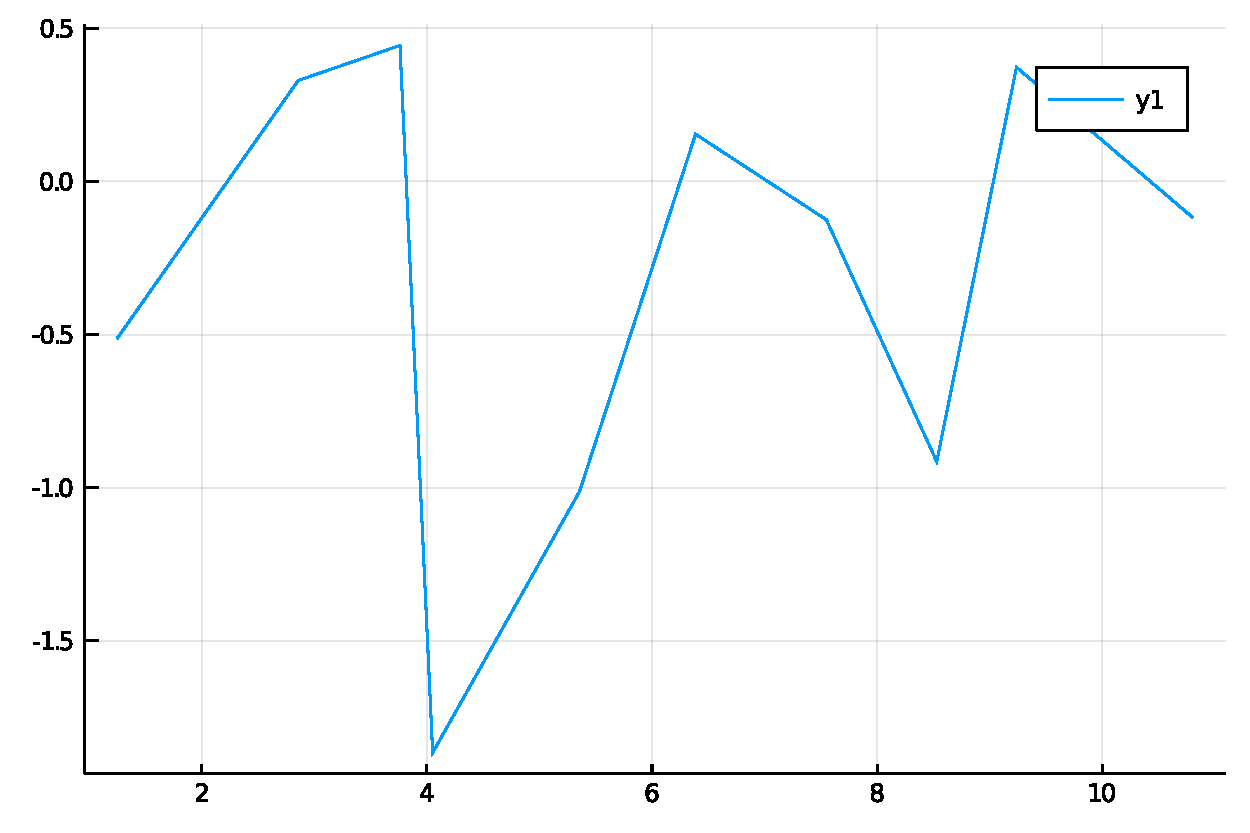
\includegraphics{hello}
  \caption{My ugly figure}
  \label{fig:hello}
\end{figure}

\section{Key concepts of the thesis}

This section provides the reader with broad explanations on the background and concepts from the thesis.
This is not yet a review of the relevant literature but a slower-paced explanation.
Ideally, this should be readable by people outside the direct thesis topic and equips them to understand the rest of the thesis.

\section{Research objectives}

We state in this section the research objectives, this does not need to be a detailed outline of the contribution chapters, since there is a dedicated chapter for this. (Summary of contributions)
         % Introduction au sujet de recherche.
% !TEX root = Document.tex

\Chapter{LITERATURE REVIEW}\label{chap:LiteratureReview}

This chapter offers an overview of the recent research on topics connected to the thesis.
This can also refer to the other chapters by highlighting the contrast with existing work.

\section{Review of recent research on the same topic}

The problem we consider was initially defined by Stackelberg in \cite{stackelberg}.

\section{Review of related methods}
 % Introduction au sujet de recherche.
% !TEX root = Document.tex

% This chapter is a requirement by Polytechnique Montreal
% only for article-based theses, i.e. theses where some chapters
% are submitted or published articles.
% you have to summarize the contributions of the different chapters,
% recall where they were published and show they form a single thesis and
% not (only) a patchwork of isolated contributions.

% If this is not a requirement from your universities,
% I would recommend adding this part as a section in the introduction instead.

\Chapter{SUMMARY OF CONTRIBUTIONS}\label{chap:WorkSynthesis}

The work presented in this thesis is structured around two aspects.
The first one is the development of a bilevel framework for the optimal
price-setting of a Time-and-Level-of-Use program. The second component is
the development of the concept of near-optimal robustness for bilevel problems.
       % Revue de littérature.
% !TEX root = Document.tex

\Chapter{CHAPTER 1}\label{chap:TLOUBilevel01}

% The tite chapter should match the title under which the article was published.
% The bibtex reference to the journal entry should also be given here.

Authors: Mathieu Besançon, Andrey Markov, published in the International Journal on Markov Chains $\left[1\right]$\footnote{\copyright 2020 Publisher. Reprinted, with permission, from $\left[1\right]$}.

\subsection*{Abstract}

This sums up our contribution.

\section{Introduction}

\section{Markov properties for unicorn transportation}\label{sec:unictransport}
               % Premier thème (Doctorat) ou "Détails de la Solution" (Maîtrise).
% !TEX root = Document.tex

\Chapter{OPTIMAL MULTI-USER UNICORN MATCHING}\label{chap:multitlou}

\section*{Abstract}

\section{Introduction}

This is a very new topic.

\section{Theory}

\begin{proposition}\label{prop:limitside}
For a capacity candidate $k \in S$, the value of the capacity has to be finite.
\end{proposition}
\begin{proof}
Argument of authority.
\end{proof}

\section{Computational experiments}\label{sec:num-resolution}

This section is mostly here to show the inclusion of a table.
I kept tables separated in the template because they are generated directly
by simulations. They are then copied to the \textit{tables} folder.

\begin{table}[]
\centering
\begin{small}
\setlength{\tabcolsep}{1.5pt}
\begin{tabular}{|l|l|l|l|l|l|l|l|l|l|l|l|l|l|}
\hline
& method & \multicolumn{4}{l|}{standard} & \multicolumn{4}{l|}{indicator} & \multicolumn{4}{l|}{lazy} \\
\hline
& nclusters & 2 & 5 & 10 & 20 & 2 & 5 & 10 & 20 & 2 & 5 & 10 & 20 \\
\hline
\multirow{5}{*}{nusers} & 5 & 10/0/0 & 10/0/0 &  -  &  -  & 10/0/0 & 10/0/0 &  -  &  -  & 10/0/0 & 10/0/0 &  -  &  -  \\
& 20 & 10/0/0 & 10/0/0 & 8/2/0 & 10/0/0 & 9/1/0 & 10/0/0 & 10/0/0 & 10/0/0 & 10/0/0 & 10/0/0 & 10/0/0 & 10/0/0 \\
& 50 & 9/1/0 & 10/0/0 & 10/0/0 & 9/1/0 & 9/1/0 & 7/3/0 & 10/0/0 & 10/0/0 & 10/0/0 & 9/1/0 & 9/1/0 & 9/1/0 \\
& 75 & 9/1/0 & 10/0/0 & 9/1/0 & 7/3/0 & 9/1/0 & 10/0/0 & 9/1/0 & 8/2/0 & 9/1/0 & 10/0/0 & 6/4/0 & 9/1/0 \\
& 100 & 9/1/0 & 10/0/0 & 6/4/0 & 8/2/0 & 10/0/0 & 9/1/0 & 7/3/0 & 8/2/0 & 8/2/0 & 10/0/0 & 10/0/0 & 9/1/0 \\
\hline
\end{tabular}
\end{small}
\caption{Feasible/Infeasible/Timed-out instances, predetermined case}
\label{tab:statspredetermined}
\end{table}


\cref{tab:statspredetermined} shows the number
of successfully optimized, infeasible, and timed-out instances for different numbers
of clusters, users, and for the three methods.
               % Second thème (Doctorat) ou "Résultats théoriques et expérimentaux" (Maîtrise).
% !TEX root = Document.tex
% This is the example of a chapter submitted as an article but not accepted yet.
% Not all chapters must be published already.

\Chapter{NEAR-OPTIMAL ROBUST BILEVEL OPTIMIZATION}\label{chap:NORBiP}

This chapter was submitted to a Journal in October 2020.

Authors: Mathieu Besançon, John von Neumann.

\subsection*{Abstract}

\section{Introduction}

\section{Model}
This section is just here to show an optimization problem, Problem \eqref{prob:foundation}.
I prefer using {subequations} for all my align environment, except when at
most one equation is numbered.

\begin{subequations}\label{prob:foundation}
\begin{align}
\min_{x,v}\,\, & F(x,v)\label{eq:NORBiPobj}\\
\text{s.t.} \,\, & G_k(x,v) \leq 0 &\forall k \in \left[\![m_u\right]\!]\label{eq:redundant} \\
& f(x,v) \leq \phi(x)\\
& g(x, v) \leq 0\\
& G_k(x,z) \leq 0\,\, \forall z \in \mathcal{Z}(x;\delta) &\forall k \in \left[\![m_u\right]\!]\label{eq:robcons}\\
& x \in \mathcal{X}.\label{eq:foundationlast}
\end{align}
\end{subequations}
               % Troisième thème (Doctorat) ou effacez ce fichier si vous êtes à la Maîtrise.
 % !TEX root = Document.tex

\Chapter{CONCLUSION}\label{chap:Conclusion}

This thesis defines new problems in constrained non-convex optimization
and applies the formulation to use cases in electricity pricing.

\section{Thesis summary}

\section{Limitations}\label{sec:Limitations}

\section{Future research}\label{sec:Future}
           % Conclusion.

%\backmatter
\ifthenelse{\equal{\Langue}{english}}{
	\renewcommand\bibname{REFERENCES}
	\bibliography{Document}
	\bibliographystyle{IEEEtran}			% Bibliography style.
}{
	\renewcommand\bibname{RÉFÉRENCES}
	\bibliography{Document}
	\bibliographystyle{IEEEtran-francais}    % Style de la bibliographie.
}

% !TEX root = Document.tex
\chapter*{RÉSUMÉ ÉTENDU}\thispagestyle{headings}
\addcontentsline{toc}{compteur}{RÉSUMÉ ÉTENDU}

Le résumé étendu en Français est conseillé par Polytechnique Montréal lorsque la
thèse est rédigée en anglais. Centrale Lille rend obligatoire un résumé étendu
lorsque la thèse est rédigée en anglais. Dans les deux cas, ce résumé étendu est
placé à la fin de la thèse, avant les références et annexes.

La thèse porte sur les modèles d'optimisation mathématiques biniveaux
et leurs applications à la réponse de la demande dans les réseaux
électriques intelligents.


\ifthenelse{\equal{\School}{centrale}}{
    % !TEX root = Document.tex

{\footnotesize
\textbf{Title: Bilevel models for demand response in smart grids}

\textbf{Titre: Modèles bi-niveaux pour la réponse de la demande dans les réseaux électriques intelligents}

\textbf{Résumé:}\\
% !TEX root = Document.tex
La thèse porte sur les modèles d'optimisation mathématique biniveau
et leurs applications à la réponse de la demande dans les réseaux
électriques.\clinebreak
L'augmentation de la production d'énergie renouvelable
et l'apparition de nouveaux acteurs ont complexifié les opérations
et décisions dans les réseaux électriques.
La nature aléatoire et distribuée de la production solaire et éolienne
entraîne un besoin d'ajustement de la production à la demande nette
correspondant à la demande après prise en compte de la production renouvelable.\clinebreak
La réponse de la demande est une des solutions utilisées pour
faire face à ces nouveaux besoins des réseaux électriques.


\textbf{Mots-clés}: \mesMotsClefFR

\textbf{Abstract:}\\
% !TEX root = Document.tex
This thesis investigates mathematical optimization models
with a bilevel structure and their application to price-based
demand response in smart grids.\clinebreak
The increasing penetration of renewable power generation
has put power systems under higher tension.
The stochastic and distributed nature of wind and solar generation
increases the need for adjustment of the production to the net demand,
which corresponds to the
demand minus the renewable generation.\clinebreak
Demand Response as a means to this adjustment of demand and
supply is receiving growing attention.


\textbf{Keywords}: \mesMotsClef
}

}{
    % if Poly then abstract already at the beginning
}


%
\ifthenelse{\equal{\AnnexesPresentes}{O}}{
	\appendix%
	\newcommand{\Annexe}[1]{\annexe{#1}\setcounter{figure}{0}\setcounter{table}{0}\setcounter{footnote}{0}}%
	% !TEX root = Document.tex

%%
%%  Appendices
%%
%%  Note: Ne pas modifier la ligne ci-dessous. / Do not modify the following line.
\ifthenelse{\equal{\Langue}{english}}{
	\addcontentsline{toc}{compteur}{APPENDICES}
}{
	\addcontentsline{toc}{compteur}{ANNEXES}
}

%%  Toutes les annexes doivent être inclues dans ce document
%%  les unes à la suite des autres.
%%  All annexes must be included in this document one after the other.

% !TEX root = Document.tex

\Annexe{MY ARTICLE IN APPENDIX}\label{chap:articleappendix}

This appendix was presented as extended abstract at, and included in the program of, the 14th Symposium on Unicorn Transportation.

Authors: Mathieu Besançon, Alan Turing.

\textbf{Summary}

This sums up the article.

\section{Introduction}

Unicorns are fun.

\section{Acknowledgment}

This work was supported by the Society of Unicorn studies.


% A second appendix (B)
\Annexe{Code examples}

\begin{verbatim}
function f(x)
    sin(x) / x
end
\end{verbatim}
}
{}
\end{document}
